\section{Scoring Rule based GAN}

\begin{frame}{Scoring Rules: Theory and Motivation}

A scoring rule $S(P^\phi, y)$ evaluates a probabilistic forecast $P^\phi$ against
an observed outcome $y$. For probabilistic forecasting, the key
property is \textbf{strict propriety}:

\begin{equation}
\begin{aligned}
\mathbb{E}_{Y\sim P^\star}
\left[S(P^\star,Y)\right]
<
\mathbb{E}_{Y\sim P^\star}
\left[S(P^\phi,Y)\right],
\qquad
P^\phi \neq P^\star .
\end{aligned}
\end{equation}

\vspace{0.1cm}

Therefore, the expected score is uniquely minimized when

\begin{equation}
P^\phi(\cdot\mid c)=P^\star(\cdot\mid c).
\end{equation}

\vspace{0.3cm}
\textbf{Why useful for probabilistic forecasting?}

\begin{itemize}
    
    \item Provides a \textbf{theoretically well-defined optimum} through
    strict propriety.
    
    \item Encourages both \textbf{accuracy and probabilistic spread},
    making it suitable for avoiding degenerate forecasts.
    
    \item Can be optimized directly with gradient-based methods using
    the generator reparameterization $Y=G_\phi(z,c)$.
\end{itemize}

\end{frame}



\begin{frame}{From ForGAN to Scoring-Rule ForGAN}

Instead of training a generator through a discriminator,
the generator directly minimizes a strictly proper scoring rule.

For the univariate forecasting \textbf{Continuous Ranked Probability Score (CRPS)}:

\begin{equation}
\begin{aligned}
&CRPS(P^\phi, y)  = \underbrace{\mathbb{E}[|X - y|]}_{\text{accuracy term}} - \frac{1}{2}\underbrace{\mathbb{E}[|X - X'|]}_{\text{spread term}} \\     
\end{aligned}
\end{equation}

With $X,X'\sim P^\phi$

\vspace{0.3cm}
\textbf{Why can this improve ForGAN?}

\begin{itemize}
    \item \textbf{Accuracy:} generated samples are pulled toward the
    observed realization through $|X-y|$.
    
    \item \textbf{Mode collapse:} a degenerate generator with
    $X\approx X'$ receives no spread reward, discouraging
    single-point forecasts.
    
    \item \textbf{No discriminator:} removes the adversarial training
    loop and its dependence on the critic's ability to provide useful
    gradients.
    
    \item \textbf{Goal:} learn the conditional distribution
    $P^\phi(\cdot\mid c)$ rather than only realistic individual samples.
\end{itemize}

\end{frame}


\begin{frame}{Scoring-Rule ForGAN Training Procedure}
    \begin{figure}[H]
    \centering
    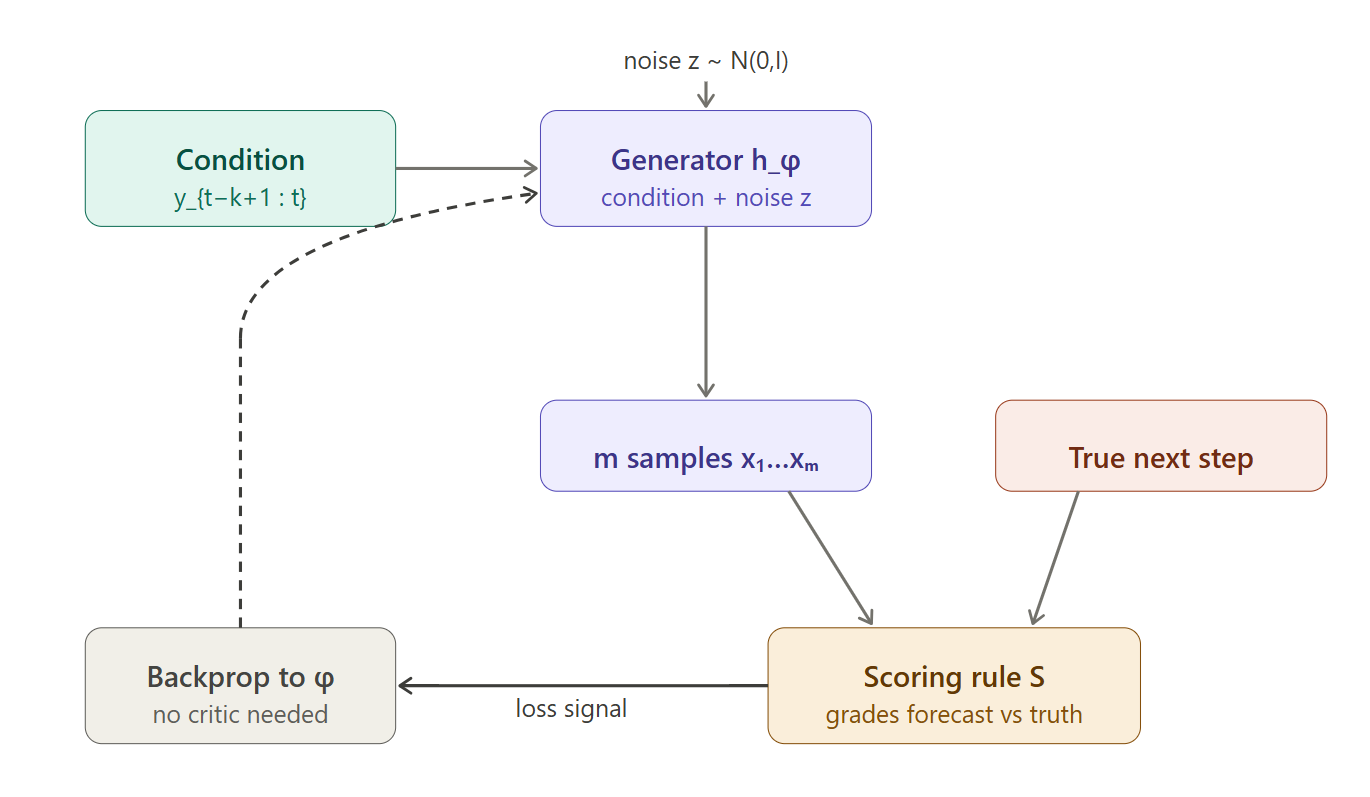
\includegraphics[scale=0.3]{images/srforgan_train_schema.png}
\end{figure}
\end{frame}